\documentclass[11pt]{article}
\usepackage{amsmath, amssymb, amsthm, enumitem, hyperref}
\usepackage{pdfpages}

% Page formatting
\usepackage[margin=1in]{geometry}
\setlength{\parskip}{0.5em}
\setlength{\parindent}{0em}

% Theorem environments
\newtheorem{theorem}{Theorem}[section]
\newtheorem{lemma}[theorem]{Lemma}
\newtheorem{corollary}[theorem]{Corollary}
\newtheorem{proposition}[theorem]{Proposition}

\theoremstyle{definition}
\newtheorem{definition}[theorem]{Definition}
\newtheorem{example}[theorem]{Example}
\newtheorem{exercise}[theorem]{Exercise}

\theoremstyle{remark}
\newtheorem{remark}[theorem]{Remark}

% Custom commands
\newcommand{\R}{\mathbb{R}}
\newcommand{\N}{\mathbb{N}}
\newcommand{\Z}{\mathbb{Z}}

% Title Page
\title{Math 51 Notes}
\author{Your Name}
\date{}

\begin{document}

\maketitle
\tableofcontents
\newpage

% Chapter 1
\section{Chapter 1: Title of Chapter 1}

\subsection{Exercise 4.1}

\begin{enumerate}
    \item[(a)] \[
\left\{
\begin{bmatrix}
x \\ y \\ z
\end{bmatrix}
\in \mathbb{R}^3 : z = 2x - y
\right\}
\]

A set of vectors \( S \subseteq \mathbb{R}^n \) is a linear subspace if and only if:
\begin{enumerate}
    \item The zero vector is in \( S \).
    \item \( S \) is closed under vector addition: if \( \mathbf{u}, \mathbf{v} \in S \), then \( \mathbf{u} + \mathbf{v} \in S \).
    \item \( S \) is closed under scalar multiplication: if \( \mathbf{u} \in S \) and \( c \in \mathbb{R} \), then \( c \cdot \mathbf{u} \in S \).
\end{enumerate}

Checking each condition:
\begin{enumerate}
    \item \textbf{The zero vector is in \( S \).}
    \[
    \mathbf{u} = 
    \begin{bmatrix} 
    0 \\ 0 \\ 0
    \end{bmatrix}
    \]
    Check if it satisfies \( z = 2x - y \): 
    \[
    2 \cdot 0 - 0 = 0.
    \]
    This is true, so the zero vector is in the set.

    \item \textbf{\( S \) is closed under vector addition.}

    Let 
    \[
    \mathbf{u} = 
    \begin{bmatrix} 
    x_1 \\ y_1 \\ z_1
    \end{bmatrix}, \quad 
    \mathbf{v} = 
    \begin{bmatrix} 
    x_2 \\ y_2 \\ z_2
    \end{bmatrix}.
    \]

    \[
    \mathbf{u} + \mathbf{v} = 
    \begin{bmatrix} 
    x_1 + x_2 \\ y_1 + y_2 \\ z_1 + z_2
    \end{bmatrix}.
    \]

    \[
    z_1 + z_2 = 2 \cdot (x_1 + x_2) - (y_1 + y_2).
    \]

    \[
    z_1 = 2 \cdot x_1 - y_1, \quad z_2 = 2 \cdot x_2 - y_2.
    \]

    \[
    z_1 + z_2 = 2 \cdot (x_1 + x_2) - (y_1 + y_2).
    \]
    Thus, the set is closed under addition.

    \item \textbf{\( S \) is closed under scalar multiplication.}

    Let
    \[
    \mathbf{u} = 
    \begin{bmatrix} 
    x  \\ y \\ z
    \end{bmatrix}.
    \]
    \[
    c \cdot \mathbf{u} = 
    \begin{bmatrix} 
    cx  \\ cy \\ cz
    \end{bmatrix}.
    \]

    \[
    cz = 2 \cdot (cx) - (cy).
    \]
    But 
    \[
    z = 2x - y.
    \]
    So 
    \[
    cz = c (2x-y) = 2 \cdot (cx) - (cy).
    \]
    Thus, the set is closed under scalar multiplication. So this is a linear subspace.
\end{enumerate}

    \item[(b)] \[
\left\{
\begin{bmatrix}
x \\ y \\ z
\end{bmatrix}
\in \mathbb{R}^3 : z = 1 + 2x - y
\right\}
\]

A set of vectors \( S \subseteq \mathbb{R}^n \) is a linear subspace if and only if:
\begin{enumerate}
    \item The zero vector is in \( S \).
    \item \( S \) is closed under vector addition: if \( \mathbf{u}, \mathbf{v} \in S \), then \( \mathbf{u} + \mathbf{v} \in S \).
    \item \( S \) is closed under scalar multiplication: if \( \mathbf{u} \in S \) and \( c \in \mathbb{R} \), then \( c \cdot \mathbf{u} \in S \).
\end{enumerate}


Checking each condition:
\begin{enumerate}
    \item \textbf{The zero vector is in \( S \).}
    \[
    \mathbf{u} = 
    \begin{bmatrix} 
    0 \\ 0 \\ 0
    \end{bmatrix}
    \]
    Check if it satisfies \( z = 1 + 2x - y \): 
    \[
    2 \cdot 0 - 0 = 1 \neq 0
    \]

This is false, so the zero vector is not in the set.
So this is not a linear subspace.
\end{enumerate}
    \item[(c)] \[
\left\{
\begin{bmatrix}
x \\ y
\end{bmatrix}
\in \mathbb{R}^2 : y = x^2
\right\}
    \]
A set of vectors \( S \subseteq \mathbb{R}^n \) is a linear subspace if and only if:
\begin{enumerate}
    \item The zero vector is in \( S \).
    \item \( S \) is closed under vector addition: if \( \mathbf{u}, \mathbf{v} \in S \), then \( \mathbf{u} + \mathbf{v} \in S \).
    \item \( S \) is closed under scalar multiplication: if \( \mathbf{u} \in S \) and \( c \in \mathbb{R} \), then \( c \cdot \mathbf{u} \in S \).
\end{enumerate}


Checking each condition:
\begin{enumerate}
    \item \textbf{The zero vector is in \( S \).}
    \[
    \mathbf{u} = 
    \begin{bmatrix} 
    0 \\ 0 
    \end{bmatrix}
    \]
    Check if it satisfies \( y = x^2 \): 
    \[
    0 = 0^2 = 0
    \]

This is true, so the zero vector is in the set.
 \item \( S \) is closed under vector addition: if \( \mathbf{u}, \mathbf{v} \in S \), then \( \mathbf{u} + \mathbf{v} \in S \).


 Let 
    \[
    \mathbf{u} = 
    \begin{bmatrix} 
    x_1 \\ y_1
    \end{bmatrix}, \quad 
    \mathbf{v} = 
    \begin{bmatrix} 
    x_2 \\ y_2
    \end{bmatrix}.
    \]

    \[
    \mathbf{u} + \mathbf{v} = 
    \begin{bmatrix} 
    x_1 + x_2 \\ y_1 + y_2
    \end{bmatrix}.
    \]

    \[
    y_1 + y_2 = (x_1 + x_2)^2
    \]
    Here
    \[
    y1 = x1^2, y2 = x2^2
    \]
    \[
    y1+y2 = x1^2 + x2^2 \neq (x1+x2)^2
    \]
\( S \) is NOT closed under vector addition. So this is not a linear subspace.
    
\end{enumerate}
    \item[(d)] \[
    \left\{
    \begin{bmatrix}
    x \\ y \\ z
    \end{bmatrix}
    \in \mathbb{R}^3 : 
    \begin{aligned}
    3x - y + z &= 0, \\
    x + y - 4z &= 0
    \end{aligned}
    \right\}
\]
A set of vectors \( S \subseteq \mathbb{R}^n \) is a linear subspace if and only if:
\begin{enumerate}
    \item The zero vector is in \( S \).
    \item \( S \) is closed under vector addition: if \( \mathbf{u}, \mathbf{v} \in S \), then \( \mathbf{u} + \mathbf{v} \in S \).
    \item \( S \) is closed under scalar multiplication: if \( \mathbf{u} \in S \) and \( c \in \mathbb{R} \), then \( c \cdot \mathbf{u} \in S \).
\end{enumerate}


Checking each condition:
\begin{enumerate}
    \item \textbf{The zero vector is in \( S \).}
    \[
    \mathbf{u} = 
    \begin{bmatrix} 
    0 \\ 0 \\ 0
    \end{bmatrix}
    \]
    Check if it satisfies 
    \[
     \begin{aligned}
    3x - y + z &= 0, \\
    x + y - 4z &= 0
    \end{aligned}
    \]
     \[
    3 \cdot 0 - 0 + 0 = 0
    \]
     \[
    0 + 0 - 4.0 = 0
    \]
    This is true, so the zero vector is in the set.
  \item 
   \item \textbf{\( S \) is closed under vector addition.}

    Let 
    \[
    \mathbf{u} = 
    \begin{bmatrix} 
    x_1 \\ y_1 \\ z_1
    \end{bmatrix}, \quad 
    \mathbf{v} = 
    \begin{bmatrix} 
    x_2 \\ y_2 \\ z_2
    \end{bmatrix}.
    \]

    \[
    \mathbf{u} + \mathbf{v} = 
    \begin{bmatrix} 
    x_1 + x_2 \\ y_1 + y_2 \\ z_1 + z_2
    \end{bmatrix}.
    \]
    \[
     \begin{aligned}
    3x - y + z &= 0, \\
    x + y - 4z &= 0
    \end{aligned}
    \]
    
    \[
     z = -3x + y \]
    \[
     z = (x+y)/4
    \]
    
    \[
    z_1 + z_2 = -3(x_1+x_2) +y
    \]
    \[
    -3(x_1)+y_1 + -3(x_2)+y_2 = -3(x_1+x_2) +y_1+y_2
    \]
    \[
    -3(x_1+x_2)+y_1+y_2 = -3(x_1+x_2) +y_1+y_2
    \]
    
    \[
    z1 + z_2 = (x_1+x_2+y_1+y_2)/4
    \]
    \[
    (x_1+y_1)/4 + (x_2+y_2)/4 = (x_1+x_2+y_1+y_2)/4
    \]
    \[
    (x_1+y_1 + x_2+y_2)/4 = (x_1+x_2+y_1+y_2)/4
    \]
    This is true so \( S \) is closed under vector addition.
    \item \textbf{\( S \) is closed under scalar multiplication.}

    Let
    \[
    \mathbf{u} = 
    \begin{bmatrix} 
    x  \\ y \\ z
    \end{bmatrix}.
    \]
    \[
    c \cdot \mathbf{u} = 
    \begin{bmatrix} 
    cx  \\ cy \\ cz
    \end{bmatrix}.
    \]
    \[
    cz = -3cx_1+cy_1
    \]
     \[
    c(-3x_1+y_1) = -3cx_1+cy_1
    \]
     \[
    -3cx_1+cy_1 = -3cx_1+cy_1
    \]

    \[
    cz_1 = (cx_1 +cy_1)/4
    \]

     \[
    c(x_1+y_1)/4 = (cx_1 +cy_1)/4
    \]
     \[
     (cx_1+cy_1)/4 = (cx_1 +cy_1)/4
    \]
     This is true so \( S \) is closed under scalar multiplication.
     So this is a linear subspace.
\end{enumerate}
\end{enumerate}

\subsection{Exercise 4.2}
For 
\[
v = 
\begin{bmatrix}
2 \\
0 \\
1
\end{bmatrix}
\quad \text{and} \quad
w = 
\begin{bmatrix}
-1 \\
1 \\
3
\end{bmatrix},
\]
find scalars $a$, $b$, $c$ so that
\[
\text{span}(v, w) = \left\{
\begin{bmatrix}
x \\
y \\
z
\end{bmatrix} \in \mathbb{R}^3 : ax + by + cz = 0
\right\}.
\]

Here 
ax + by + cz = 0

From \[
v = 
\begin{bmatrix}
2 \\
0 \\
1
\end{bmatrix}
\]
we have 
\[
a(2) + 0(b) + 1(c) = 0
\]
\[
c = -2(a)
\]

From \[
w = 
\begin{bmatrix}
-1 \\
1 \\
3
\end{bmatrix}
\]
we have 
\[
a(-1) + 1(b) + 3(c) = 0
\]
\[
b = a-3c
\]
Therefore we have scalars a,b,c such that 
\[
 b= a-3c
 \]
\[ c = -2a
\]
Substituting a =1
\[
c=-2
\]
\[
b = 1-3(-2.1) = 7
\]
Substituting we have 
\[
1(x) + 7(y) + -2(z) = 0
\]

From \[
v = 
\begin{bmatrix}
2 \\
0 \\
1
\end{bmatrix}
\]
\[
1(x) + 7(y) + -2(z) = 0
\]
we have 
\[
1(2) + 7(0) + -2(1) = 2 - 2 =0
\]


From \[
w = 
\begin{bmatrix}
-1 \\
1 \\
3
\end{bmatrix}
\]

we have
\[
1(x) + 7(y) + -2(z) = 0
\]
\[
1(-1) + 7(1) + -2(3) 
\]
\[
= -1 + 7 + -6 = -7 + 7 = 0
\]
The resulting triplets work.
\subsection{Exercise 4.3}


For 
\[
v = 
\begin{bmatrix}
1 \\
1 \\
1
\end{bmatrix}
\quad \text{and} \quad
w = 
\begin{bmatrix}
4 \\
2 \\
1
\end{bmatrix},
\]
find scalars $a$, $b$, $c$ so that
\[
\text{span}(v, w) = \left\{
\begin{bmatrix}
x \\
y \\
z
\end{bmatrix} \in \mathbb{R}^3 : ax + by + cz = 0
\right\}.
\]

For 
\[
v = 
\begin{bmatrix}
1 \\
1 \\
1
\end{bmatrix}
\quad \text{and} \quad
w = 
\begin{bmatrix}
4 \\
2 \\
1
\end{bmatrix},
\]
find scalars $a$, $b$, $c$ so that
\[
\text{span}(v, w) = \left\{
\begin{bmatrix}
x \\
y \\
z
\end{bmatrix} \in \mathbb{R}^3 : ax + by + cz = 0
\right\}.
\]

Here 
ax + by + cz = 0

From \[
v = 
\begin{bmatrix}
1 \\
1 \\
1
\end{bmatrix}
\]
we have 
\[
a(1) + 1(b) + 1(c) = 0
\]
\[
b = -(a+c)
\]

From \[
w = 
\begin{bmatrix}
4 \\
2 \\
1
\end{bmatrix}
\]
we have 
\[
a(4) + 2(b) + 1(c) = 0
\]
\[
c = -(4a+2b)
\]
Therefore we have scalars a,b,c such that 
\[
 b= -(a+c)
 \]
\[ c = -(4a+2b)
\]
Substituting a =1 and solving for b and c we get
\[
c=2
\]
\[
b =-3
\]
Substituting we have 
\[
1(x) -3(y) + 2(z) = 0
\]

From \[
v = 
\begin{bmatrix}
1 \\
1 \\
1
\end{bmatrix}
\]
\[
1(x)-3(y) + 2(z) = 0
\]
we have 
\[
1(1) -3(1) + 2(1) = 3 - 3 =0
\]


From \[
w = 
\begin{bmatrix}
4 \\
2 \\
1
\end{bmatrix}
\]

we have
\[
1(x) -3(y) + 2(z) = 0
\]
\[
1(4) + -3(2) + 2(1)
\]
\[
= 6 - 6 = 0
\]
The resulting triplets work.
\subsection{Exercise 4.4}
For the 4-vectors 
\[
w = 
\begin{bmatrix}
-2 \\
2 \\
1 \\
1
\end{bmatrix}
\quad \text{and} \quad
w' = 
\begin{bmatrix}
3 \\
4 \\
0 \\
1
\end{bmatrix},
\]
show that the collection of vectors
\[
V = \left\{ 
x = 
\begin{bmatrix}
x_1 \\
x_2 \\
x_3 \\
x_4
\end{bmatrix} 
\in \mathbb{R}^4 : x \cdot w = 0, \, x \cdot w' = 0
\right\}
\]
is a linear subspace of $\mathbb{R}^4$ in each of the following ways:

\begin{enumerate}
    \item[(a)] For $x \in V$, solve for each of $x_3$ and $x_4$ in terms of $x_1$ and $x_2$ to write $V$ as a span of two vectors;
    \item[(b)] For $x \in V$, solve for each of $x_1$ and $x_4$ in terms of $x_2$ and $x_3$ to write $V$ as a span of two vectors.
\end{enumerate}

Solution:
\begin{enumerate}


\item[(a)] For \(w\),
\[
w \cdot x = -2x_1 + 2x_2 + x_3 + x_4 = 0 \quad \Rightarrow \quad x_3 + x_4 = 2x_1 - 2x_2 \tag{1}
\]
For \(w'\),
\[
w' \cdot x = 3x_1 + 4x_2 + x_4 = 0 \quad \Rightarrow \quad x_4 = -3x_1 - 4x_2 \tag{2}
\]
Substitute \(x_4\) from (2) into (1):
\[
x_3 + (-3x_1 - 4x_2) = 2x_1 - 2x_2
\]
\[
x_3 = 5x_1 + 2x_2 \tag{3}
\]
Thus, the components of \(x\) are:
\[
x_3 = 5x_1 + 2x_2, \quad x_4 = -3x_1 - 4x_2
\]
Substitute these into \(x\):
\[
x =
\begin{bmatrix}
x_1 \\
x_2 \\
5x_1 + 2x_2 \\
-3x_1 - 4x_2
\end{bmatrix}
= x_1
\begin{bmatrix}
1 \\
0 \\
5 \\
-3
\end{bmatrix}
+ x_2
\begin{bmatrix}
0 \\
1 \\
2 \\
-4
\end{bmatrix}
\]
The basis vectors are:
\[
\begin{bmatrix}
1 \\
0 \\
5 \\
-3
\end{bmatrix}, \quad
\begin{bmatrix}
0 \\
1 \\
2 \\
-4
\end{bmatrix}.
\]

\item[(b)] For \(w\),
\[
w \cdot x = -2x_1 + 2x_2 + x_3 + x_4 = 0 \quad \Rightarrow \quad x_4 = -2x_1 + 2x_2 - x_3 \tag{4}
\]
For \(w'\),
\[
w' \cdot x = 3x_1 + 4x_2 + x_4 = 0 \quad \Rightarrow \quad x_4 = -3x_1 - 4x_2 \tag{5}
\]
Equating \(x_4\) from (4) and (5):
\[
-2x_1 + 2x_2 - x_3 = -3x_1 - 4x_2
\]
Simplify:
\[
x_1 + 6x_2 - x_3 = 0 \quad \Rightarrow \quad x_1 = -6x_2 + x_3 \tag{6}
\]
Substitute \(x_1\) from (6) into (4):
\[
x_4 = -2(-6x_2 + x_3) + 2x_2 - x_3
\]
\[
x_4 = 12x_2 - 2x_3 + 2x_2 - x_3
\]
\[
x_4 = 14x_2 - 3x_3 \tag{7}
\]
Thus, the components of \(x\) are:
\[
x_1 = -6x_2 + x_3, \quad x_4 = 14x_2 - 3x_3
\]
Substitute these into \(x\):
\[
x =
\begin{bmatrix}
-6x_2 + x_3 \\
x_2 \\
x_3 \\
14x_2 - 3x_3
\end{bmatrix}
= x_2
\begin{bmatrix}
-6 \\
1 \\
0 \\
14
\end{bmatrix}
+ x_3
\begin{bmatrix}
1 \\
0 \\
1 \\
-3
\end{bmatrix}
\]
The basis vectors are:
\[
\begin{bmatrix}
-6 \\
1 \\
0 \\
14
\end{bmatrix}, \quad
\begin{bmatrix}
1 \\
0 \\
1 \\
-3
\end{bmatrix}.
\]

\end{enumerate}
\subsection{Exercise 4.5}


Find a nonzero 3-vector \(\mathbf{v}\) so that
\[
\left\{
\mathbf{x} \in \mathbb{R}^3 : \mathbf{x} \cdot 
\begin{bmatrix}
3 \\
2 \\
1
\end{bmatrix} 
= 0, \, 
\mathbf{x} \cdot 
\begin{bmatrix}
-2 \\
-1 \\
1
\end{bmatrix} 
= 0
\right\}
= \text{span}(\mathbf{v}).
\]
Then, using the \textit{geometric} fact that any two different planes through the origin in \(\mathbb{R}^3\) meet along a line through the origin, interpret this algebraic outcome that the left side is the span of a single vector.

Solution:

Let a,b,c be scalar so that 

\[
3a+2b+c=0
\]
\begin{equation}
    b = \frac{-c-3a}{2}
\end{equation}
\[
-2a-b+c=0
\]
\[
-2a- \frac{-c-3a}{2}+c=0
\]
\[
c=\frac{a}{3}
\]
\[
2b=-\frac{a}{3}-3a
\]
\[
b=-\frac{5a}{3}
\]
writing v in terms of a,
\[
\begin{bmatrix}
a \\
-\frac{5a}{3} \\
\frac{a}{3}
\end{bmatrix} 
\]

\[
v =
a .  \begin{bmatrix}
1\\
-\frac{5}{3} \\
\frac{1}{3}
\end{bmatrix} 
\]
The two planes defined by the equations
\begin{equation}
    3a+2b+c=0
\end{equation}
\begin{equation}
    -2a-b+c=0
\end{equation}
intersect along a line through the origin in \(\mathbb{R}^3\)
This line is spanned by the vector v. Hence, the solution set is
\[
a .  \begin{bmatrix}
1\\
-\frac{5}{3} \\
\frac{1}{3}
\end{bmatrix} 
\]
Here a $\neq$ 0
so the span is
\[
\begin{bmatrix}
1\\
-\frac{5}{3} \\
\frac{1}{3}
\end{bmatrix} 
\]
\subsection{Exercise 4.6}
 Find a pair of 3-vectors \(\mathbf{v}, \mathbf{w}\) so that
\[
\left\{
\begin{bmatrix}
x \\
y \\
z
\end{bmatrix}
\in \mathbb{R}^3 : 2x - 3y + 2z = 0
\right\}
= \text{span}(\mathbf{v}, \mathbf{w}).
\]


we have 
\[
 2x - 3y + 2z = 0
\]
 Therefore
\[
 x  = \frac{3y-2z}{2}
\]
we can write x=
\[
\begin{bmatrix}
x \\
y \\
z
\end{bmatrix}
\]
as x=
\[
\begin{bmatrix}
\frac{3y-2z}{2} \\
y \\
z
\end{bmatrix}
\]
x= 
\[
y 
\begin{bmatrix}
\frac{3}{2} \\
1 \\
0
\end{bmatrix}
+ z
\begin{bmatrix}
-1 \\
0 \\
1
\end{bmatrix}
\]
Two linearly independent vectors spanning the subspace are:

\[
v1=
\begin{bmatrix}
\frac{3}{2} \\
1 \\
0
\end{bmatrix}
\]
and
\[
 v2=
\begin{bmatrix}
-1 \\
0 \\
1
\end{bmatrix}
\]
\subsection{Exercise 4.7}
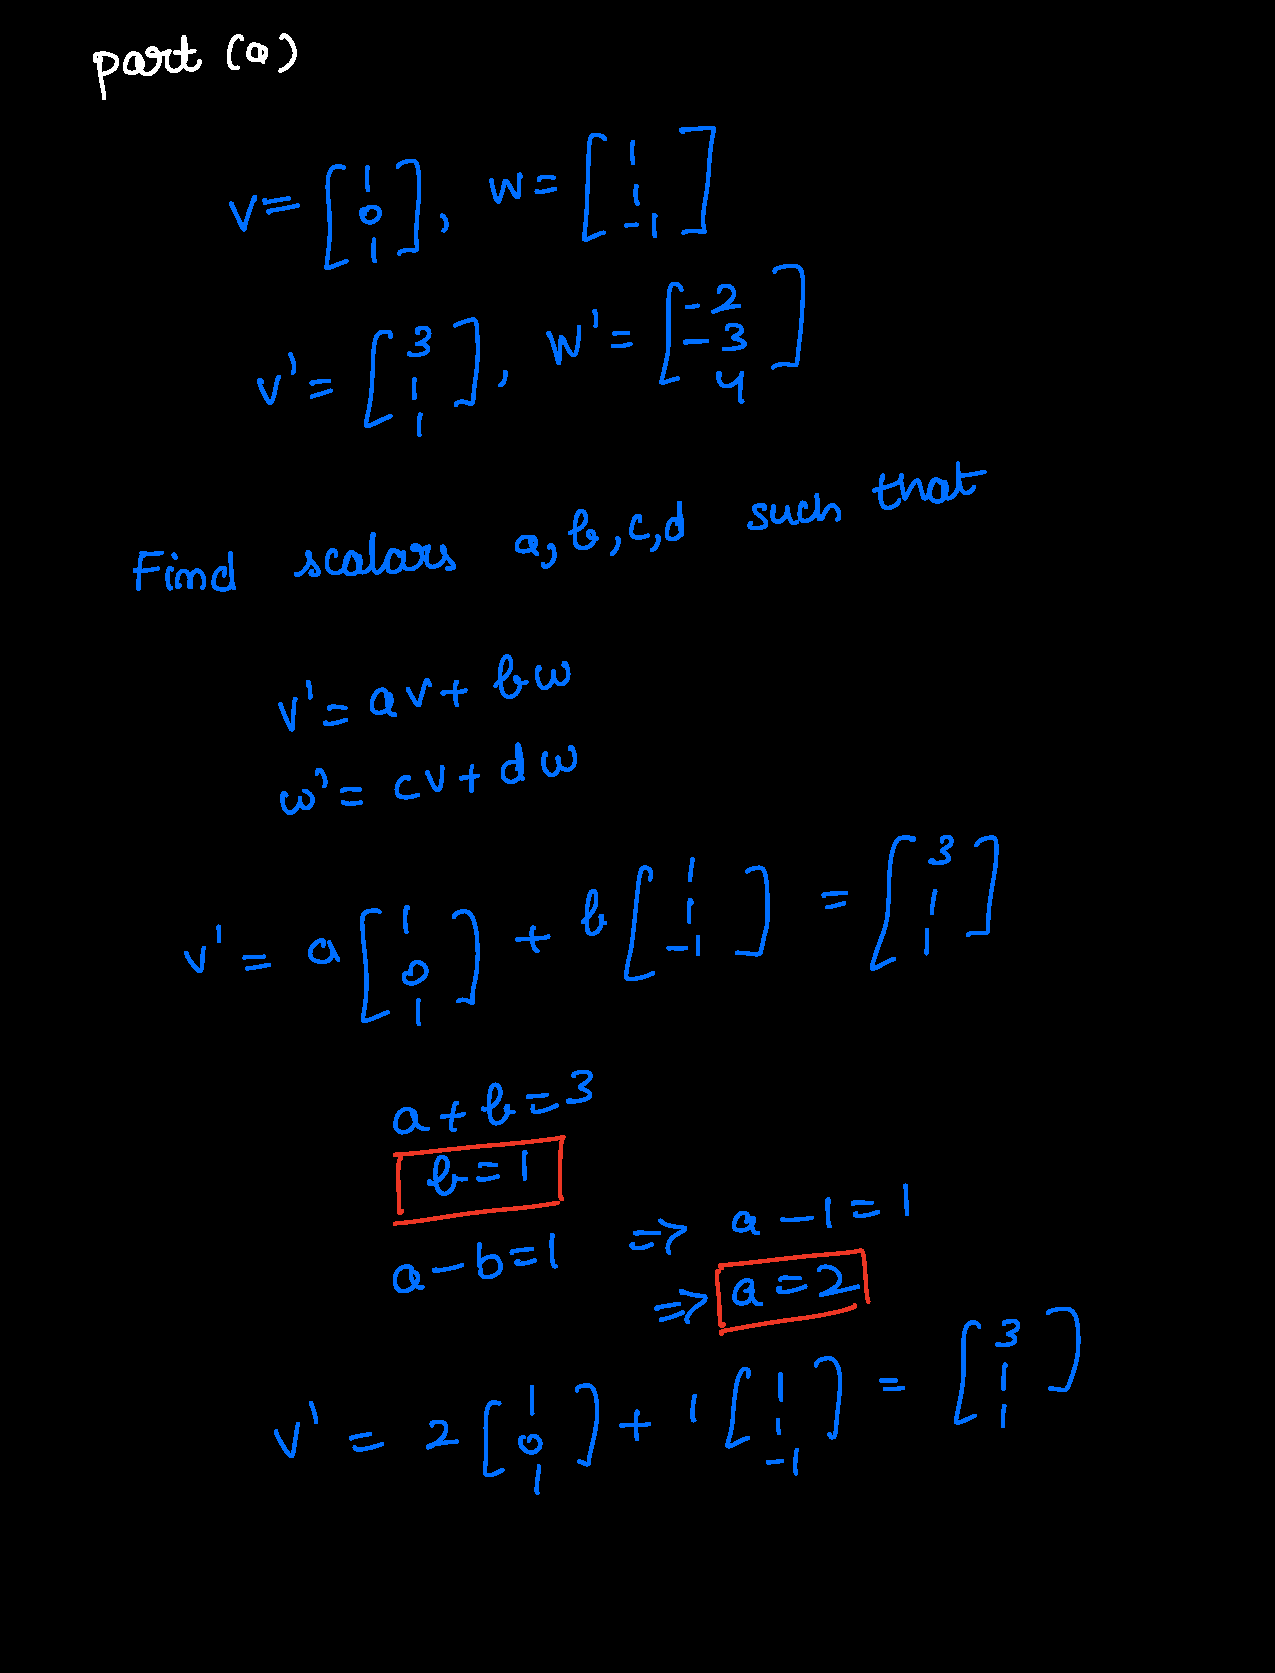
\includepdf[pages=-]{exercises/exercise_4_7.pdf}
\end{document}
